\setauthor{Moritz Eder}

In der heutigen Welt entstehen immer mehr Termine für Besprechungen oder Meetings. 
Dadurch wird es der generelle Alltag hektischer und schneller, was sowohl oft im Arbeitsleben, als auch im 
privaten Bereich zutrifft. Daher empfinden viele Menschen den Ablauf des Tages persönlich als stressig.

Oft fehlt daher die Möglichkeit sich zu entspannen und die Betroffenen verlieren den Mut sich
Hilfe zu holen.

Stress oder Leistungsdruck kann neben einem Burnout auch noch weitere gesundheitliche Folgen hervorrufen.
Mögliche Folgen von hohem Stress oder hohem Leistungsdruck könnten sein:

\begin{itemize}
    \item Zeichen von Nervosität
    \item Verspannungen, die zu Kopf-, Genick- und Rückenschmerzen führen können
    \item Vergesslichkeit
    \item Depressionen
    \item Psychische Störungen
\end{itemize}

Anhaltender Stress kann auch zu dauerhaften Herz/Kreislauf- und Nierenerkrankungen, Stoffwechselstörungen, 
Allergien oder Entzündungskrankheiten führen. \cite{stress} 
Gesundheit ist ein sehr wichtiger Faktor, deswegen benötigen gestresste Menschen eine Möglichkeit sich
wieder entspannen zu können.

\begin{figure}[H]
    \centering
    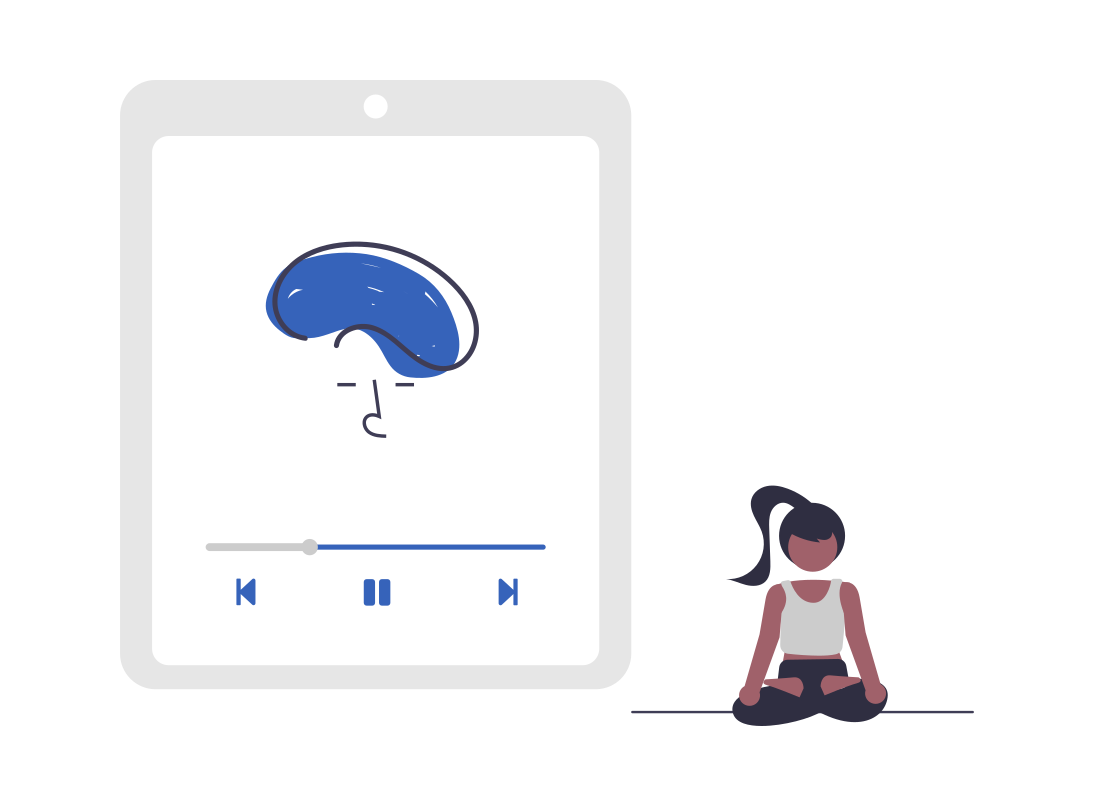
\includegraphics[height=0.35\textwidth]{./pics/undraw_Meditating_re_aiqa.png}
    \caption{Musik dient zur Entspannung}
\end{figure}

